\section{Rechner-Architekturen}
Als \textbf{Mikroprozessorarchitektur} bezeichnet man die übergreifende, von Einzelheiten abstrahierende Darstellung des inneren Aufbaus von Mikroprozessoren.
Dabei unterscheidet man zwischen dem \textbf{Operationsprinzip} (funktionelles Verhalten) und dem \textbf{Programmiermodell} (Registerbreite und Organisation, Register, Adressierungsarten, Instruktionsset, Kodierung+Dekodierung).

\subsection{Architekturklassen}
%{\large{\textbf{Architekturklassen}}}\\
\begin{itemize}[noitemsep,topsep=0pt]
	\item Stack-Architektur:\\
	Quell- und Zieloperanden sind auf dem Stack gespeichert und es wird dort auf sie zugegriffen (Operationen sind Stack-Orientiert).\\
	+ Keine explizite Angabe von Operanden notwenig $\rightarrow$ minimale Op-Codlänge für Arithmetikbefehle\\
	- Umfangreiche Austauschoperationen vom und zum Stack notwendig $\rightarrow$ wachsende Codegrösse
	
	\item Akkumulator Architektur:\\
	Ein oder wenige Akkumulatoren als zentrale Register. In der Befehlscodierung wird bereits implizit festgelegt, welches Register als Quelle und ggf. Ziel genutzt wird.\\
	+ Teilweise implizite Operandenangabe möglich, einfachste Architektur, Verzicht auf Stack möglich\\
	- zentrales Register wird sehr stark genutzt, daher ggf. Engmass mit Notwwndigkeit zur Zwischenspeicherung.
	
	\item Register-Speicher-Architektur:\\
	Erweiterung der Akkumulator-Architektur; Register als auch Speicheradresse werden explizit angegeben.\\
	+ Daten können ohne Ladezugriff für Operationen genutzt werden.\\
	- Ladezugriffe im Speicherbereich benötigen wesentlich mehr Zeit als Registerzugriff
	
	\item Load-Store-Architektur (RISC-Architekturen werden so gemacht):\\
	Es gibt ausschliesslich ein Interface zwischen den Prozessor-internen Registern und dem externen Speicher. Operationen zur Verknüpfung von Daten wirken nur zwischen den Registerinhalten.\\
	+ Schnellstmögliche Operationen durch Registeroperanden\\
	- Explizite Ladezugriffe notwendig, Codegrösse wächst
\end{itemize}

\subsection{Klassifikations-Schemata}
%{\large{\textbf{Klassifikations-Schemata}}}\\
\textbf{Duales Unterscheidungskriterium (Klassierung nach Flynn)}
\begin{figure}[htbp]
	
	\begin{minipage}{0.45\textwidth}		
		\begin{enumerate}[noitemsep,topsep=0pt]
			\item Wie viele Instruktionen werden gleichzeitig ausgeführt: Anzahl Datenströme und bearbeitete Befehle (SI: Single Instruction, MI: Multi Instruction, SD: Single Data, MD Mul)?
			
			\item Wie viele Datenwerte verarbeitet eine Instruktion?
		\end{enumerate}	
	\end{minipage}
	\hfill		
	\begin{minipage}{0.5\textwidth} 
		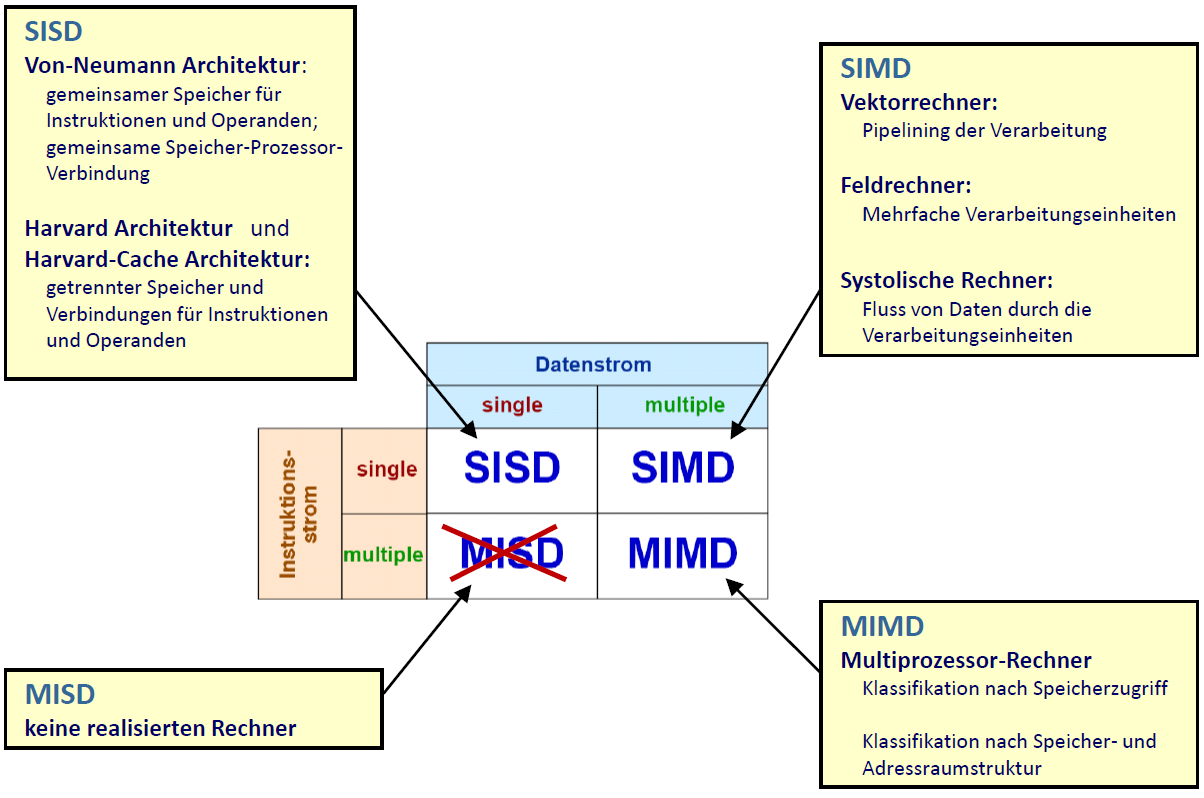
\includegraphics[width=\textwidth]{images/Rechnerarchitekturen/Klassierung_uP.PNG}
	\end{minipage}
	
\end{figure}

\textbf{Merkmale MIMD Rechnern}

\begin{itemize}[noitemsep,topsep=0pt]
	\item Homogenität der Prozessoren:\\
	Ein Multiprozessor-System ist homogen, wenn alle Prozessoren des Systems hardwaremässig gleich aufgebaut sind.
	
	\item Aufgabenstellung:\\
	Beim assymetrischen Multi-Prozessorsystem übernimmt ein Prozessor (als Master) die Steuerung aller beteiligten Prozessoren.
	Beim Symmetrischen Multiprozessorsystem übernimmt jeder Prozessor nur eine Aufgabe.
	
	\item Kopplung der Prozessoren:\\
	Enge Kopplung (alle Prozessoren haben Zugriff auf einen gemeinsamen Speicher), Schwache Kopplung (die einzelnen Prozessoren nutzen eine Kommunikationseinrichtung für den Informationsaustausch)
	
	\item Anzahl der Prozessoren
\end{itemize}

\subsection{Amdahl's Law}
%{\large{\textbf{Amdahl's Law}}}\\

Das Amdahlsche Gesetz ist ein Modell über die Beschleunigung von Programmen durch parallele Ausführung.
Nach Amdahl wird der Geschwindigkeitszuwachs vor allem durch den sequentiellen Anteil ($s$ in \%) des Problems beschränkt, da sich dessen Ausführungszeit durch Parallelisierung (Anzahl SISD-Prozessoren $n$) nicht verringern lässt.

\begin{figure}[ht]
	\begin{minipage}[t]{0.475\textwidth}
\begin{equation*}
Speedup = \dfrac{1}{s+ \dfrac{1-s}{n}}
\end{equation*}
	\end{minipage}
	\hfill
	\begin{minipage}[t]{0.475\textwidth}
		$Speedup$: Leistungssteigerung\\
		$s$      : Serieller Anteil der Arbeit\\
		$n$      : Anzahl SISD-Prozessoren
	\end{minipage}	
\end{figure}

\begin{figure}[ht]
	\begin{minipage}[t]{0.475\textwidth}
		\begin{equation*}
			T_m = \dfrac{A}{L_{SISD}} \cdot \left( s + \dfrac{p}{n} \right)
		\end{equation*}
	\end{minipage}
	\hfill
	\begin{minipage}[t]{0.475\textwidth}
		$T_m$: Totale Ausführzeit\\
		$A$      : Arbeit (Arbeitsschritte)\\
		$L_{SISD}$: Leistung SISD-Rechners\\
		$s$      : Serieller Anteil der Arbeit\\
		$p$      : Paralleler Anteil der Arbeit\\
		$n$      : Anzahl SISD-Prozessoren
	\end{minipage}	
\end{figure}

Zur Lösung von mathematischer Probleme im n-dimensionalen Raum (z.B. rechenintensive Datenverarbeitungen, Wettervorhersagemodelle) sind Multi-Prozessorsysteme fast ideal.
Sind sehr viele kleinere, von einander unabhängige Programme auszuführen, so eignet sich die Bauform MIMD ebenfalls.

\subsection{CISC/RISC Charakterisierung}
%{\large{\textbf{CISC/RISC Charakterisierung}}}\\

Bis zu ca. 1980 gab es die Tendenz, immer mehr umfangreichere und komplexere Instruktionen für $\mu$Ps bereitzustellen.
Studien besagen jedoch, dass $10\%$ der Befehle $80\%$ des Programmcodes und $21\%$ der Befehle $95\%$ des Programmcodes ausmachen.
Deshalb kam man immer mehr zu den RISC-Architekturen.
Bei diesen will man möglichst kurze und effizienze (1 Clock per Instruction CPI) Befehle haben.

\begin{table}[ht]
	\centering
	\begin{tabular}{ |p{10 cm} |p{2 cm}|p{4 cm}|}
		\hline				%& \hline	\\
		\textbf{Merkmale} 	& 	\textbf{RISC}	& \textbf{CISC} \\
		\hline Anzahl Maschinenbefehle	& $\leqq 150$	& $\geqq 200$ \\
		Anzahl der Adressierungsmodi	& $\leqq 4$ 	& viele \\
		Anzahl der Befehlsformate 		& $\leqq 4$ 	& viele \\
		Anzahl der allgemeinen CPU Registern & $\geqq 32$ 	& $\leqq 32$ \\
		Ausführung aller oder der meisten Maschinenbefehle in einem Zyklus 		& ja 	& mehrere Taktzyklen \\	
		Speicherzugriff über Load/Store-Befehle & ja & raffinierte Zugriffe \\
		Festverdrahtete Steuerung		& ja	& Mikro-programm \\
		Unterstützung höherer Programmiersprache & ja 	& ja \\
		Semantische Lücke				& gross			& klein \\
		\hline
	\end{tabular} 

\end{table}

Eine allgemein anerkannte, einfache Definition für RISC-Prozessoren existiert nicht.
Wenn der Prozessor $5$ der $8$ RISC-Merkmalen erfüllt, kann man sagen, dass es sich um einen RISC-Prozessor handelt. 

\subsection{Pipeline-Architekturen}
%{\large{\textbf{Pipeline-Architekturen}}}\\
Die Grundidee einer Pipeline-Architektur ist die, dass die verschiedenen Bearbeitungspahsen so gewählt werden, dass pro Phase etwa die gleiche Zeit benötigt wird.
Die Ausführungs eines Befehls dauert mehrere Taktzyklen, dafür werden mehrere Befehle gleichzeitig ausgeführt.
Bei jedem Takt wird somit ein Befehl abgeschlossen.
Die Anzahl Pipline-Stufen variieren je nach Prozessortyp, oftmals sind es die fünf Phasen: Fetch, Decode, Execute, Memory Access (Zugriff auf Register) und Write Back (Resultat in Speicher schreiben).
\begin{figure}[htbp]
	
	\begin{minipage}{0.5\textwidth}
		Die Befehlsdaten werden zwischen den einzelnen Befehlsphasen in Pipelineregistern zwischengespeichert. Sie sind füd den Nutzer nicht sichtbar und gelten als limitierenden Faktor bezüglich der Geschwindigkeit		
		
	\end{minipage}
	\hfill		
	\begin{minipage}{0.45\textwidth} 
		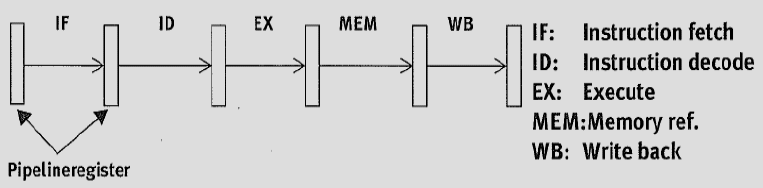
\includegraphics[width=\textwidth]{images/Rechnerarchitekturen/Pipeline.PNG}
	\end{minipage}
	
\end{figure}

Die Geschwindigkeit wird durch folgende Punkte limittiert:
\begin{itemize}[noitemsep,topsep=0pt]
	\item Buszugriffzeiten
	\item Verzögerung durch Pipelineregister
	\item Ressourcenkonflikte (strukturelle Hazards)
	\item Störungen im Kontrollfluss
	\item Störungen im Datenfluss (Datenkonflikte, Data Hazards)
\end{itemize}

\subsection{Hazards}
\subsubsection{Data Hazards}
\begin{itemize}[noitemsep,topsep=0pt]
	\item Write-After-Write-Hazard (WAW):\\
	Die Reihenfolge der Schreiboperationen muss exakt eingehalten werden
	\item Read-After-Write-Hazard (RAW):\\
	Daten dürfen erst gelesen (und) verwendet werden, wenn sie berechnet und im Register gespeichert sind. Tritt häufiger auf als WAW, erfordert Wartezyklen
\end{itemize}

\textbf{Pipeline Stall:}\\
Es resultiert ein Pipeline Stall wenn ein nachfolgebefehl das Resultat vom vorgängigen Befehl benötigt, dieser das Resultat jedoch noch nicht fertig berechnet hat

\textbf{Data-Forwarding:}\\
Resultate werden einer nachfolgenden Pipelinestufe direkt bereitgestellt, noch bevor diese an die endgültige Stelle geschrieben werden.
Neben einem Register wird der berechnete Wert gerade wieder der ALU zur Verfügung gestellt.
Somit kann direkt Execute ausgeführt werden.

\subsubsection{Kontrollflusshazards}
Verzweigungs- (Branch-) und Sprung- (Jump-) Befehle beeinflussen den sequentiellen Programmablauf.
Je nach dem muss die Pipeline geleert (Pipeline-Flush) werden, was das Programm wiederum langsam macht.
Man versucht deshalb entweder das Sprungziel parallel in einer Additionseinheit zu berechnen \textbf{(Look-Ahead Resolution)}, Wartezyklen zu vermeiden (Delay-Slot, allenfalls NOP) oder eine Verzweigungsvorhersage zu machen.

\begin{figure}[htbp]
	
	\begin{minipage}{0.55\textwidth}
		\begin{itemize}[noitemsep,topsep=0pt]
			\item Statische vorhersage:\\
			 Vorwärtssprünge $\rightarrow$ Branch not taken\\ Rückwärtssprünge $\rightarrow$ Branch taken
			 
			 \item Dynamische Vorhersage:\\
			 Aufgrund unmittelbarer Vergangenheit, siehe Abb.
			 
			 \item Korrelations-basierte Vorhersage:\\
			 Branch History Table (BHT)\\
			 Branch History Register (BHR)\\
			 Pattern History Table (PHT)

		\end{itemize}
			
		
	\end{minipage}
	\hfill		
	\begin{minipage}{0.4\textwidth} 
		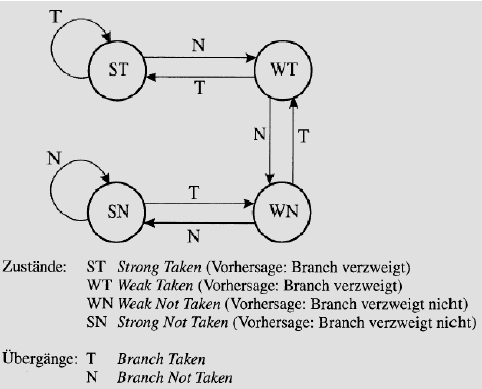
\includegraphics[width=\textwidth]{images/Rechnerarchitekturen/Sprungvorhersage.PNG}
	\end{minipage}
	
\end{figure}

\subsection{Superskalare Prozessoren}
\textbf{Skalare Architekturen:}\\
Pro Taktzyklus wird ein Befehl ausgeführt (RISC Architekturen)

\textbf{Superskalare Architekturen:}\\
Bei Superskalarität kann pro Zxklus mehr als ein Befehl abgearbeitet werden.
Da Befehle gleichzeitig starten (und enden) enstehen Schwierigkeiten und Gefahren:
\begin{itemize}[noitemsep,topsep=0pt]
	\item Invertierte zeitliche Reihenfolge (out of order execution)
	\item Sprung- und Verzweigungsvefehle wirken sich noch dramatischer aus als bei einfachen Pipelines, NOPs sind kaum noch vertretbar
	\item Datenabhängigkeiten wirken sich ebenfalls drastisch aus (out of order execution)
			
\end{itemize}
%\todo{ev ergänzen}

\textbf{Superskalare Pipeline:}\\
Befehle werden gleichzeitig abgearbeitet

\textbf{Superpipeline:}\\
Befehle werden in feiner granulierte Elemente aufgeteilt. Dadurch wird die Hardware grösser, da mehr Transferregister benötigt werden.\newline

Ebenfalls gibt es diverse Mischvarianten.

\subsection{Very Long Instruction Word- (VLIW-) Prozessoren}
VLIW Prozessoren können als Variation der superskalaren Prozessoren gesehen werden

\begin{figure}[htbp]
	
	\begin{minipage}{0.55\textwidth}
		\begin{itemize}[noitemsep,topsep=0pt]
			\item Mehrere Mschinenbefehle werden in einem Instruktionswort gespeichert.
			\item Compiler nimmt mehrere Befehle und setzt sie zu einem grossen Befehl zusammen. Befehl kann effizienter abgearbeitet werden.
			
		\end{itemize}
		
	\end{minipage}
	\hfill		
	\begin{minipage}{0.4\textwidth} 
		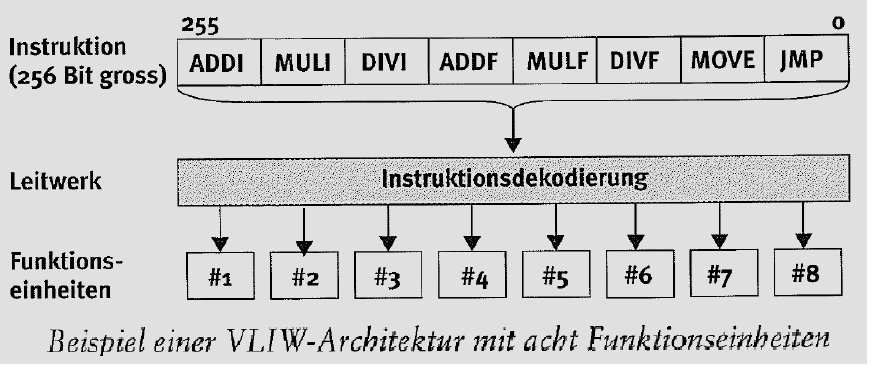
\includegraphics[width=\textwidth]{images/Rechnerarchitekturen/VILW.PNG}
	\end{minipage}
	
\end{figure}

\subsection{Explicit Parallel Instruction Computing- (EPIC-) Architektur}
 
\begin{figure}[htbp]
	
	\begin{minipage}{0.55\textwidth}
Die EPIC-Architektur ist ein  Spezialfall der VILW-Konzepts. Bei der Programmierung von EPIC-CPUs wird die Parallelisierung der Befehle eines Instruktionsstromes explizit vorgenommen. Die ISA hat Eigenschaften, die die explizite Parallelisierung unterstützen, während eine herkömmliche ISA von einer sequentiellen Abarbeitung der Befehle ausgeht.
		
	\end{minipage}
	\hfill		
	\begin{minipage}{0.4\textwidth} 
		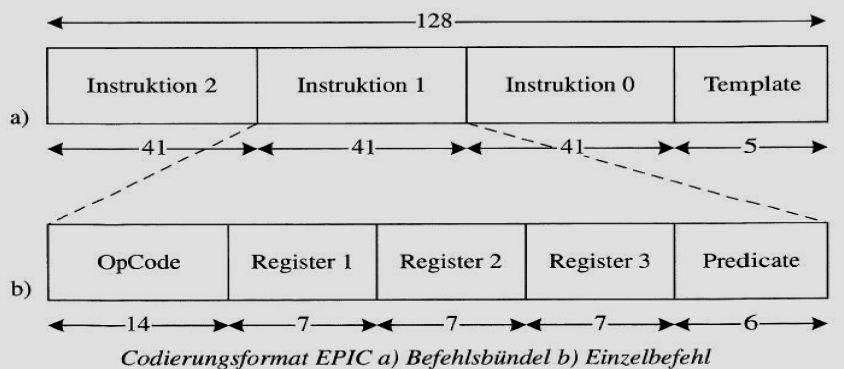
\includegraphics[width=\textwidth]{images/Rechnerarchitekturen/EPIC.PNG}
	\end{minipage}
	
\end{figure}
%\todo{Ev ergänzen oder anders. keine ahnung}

\subsection{Leistungsbewertung von Rechnern}
Das am meisten interessierende Leistungsmerkmal eines Einzel-Prozessors ist die für die Ausführung eines bestimmten Programms benötigte Zeit:
\begin{equation*}
	t_A = n_I \cdot c_I \cdot t_I = n_I \cdot c_I \cdot \dfrac{1}{f_{clk}}
\end{equation*}
Wobei $n_I$ die Anzahl der ausgeführten Instruktionen, $c_I$ die mittlere Anzahl benötigte Taktzyklen pro Instruktion (CPI) und $t_I$ die Zeit pro Taktperiode ist.

\begin{figure}[ht]
	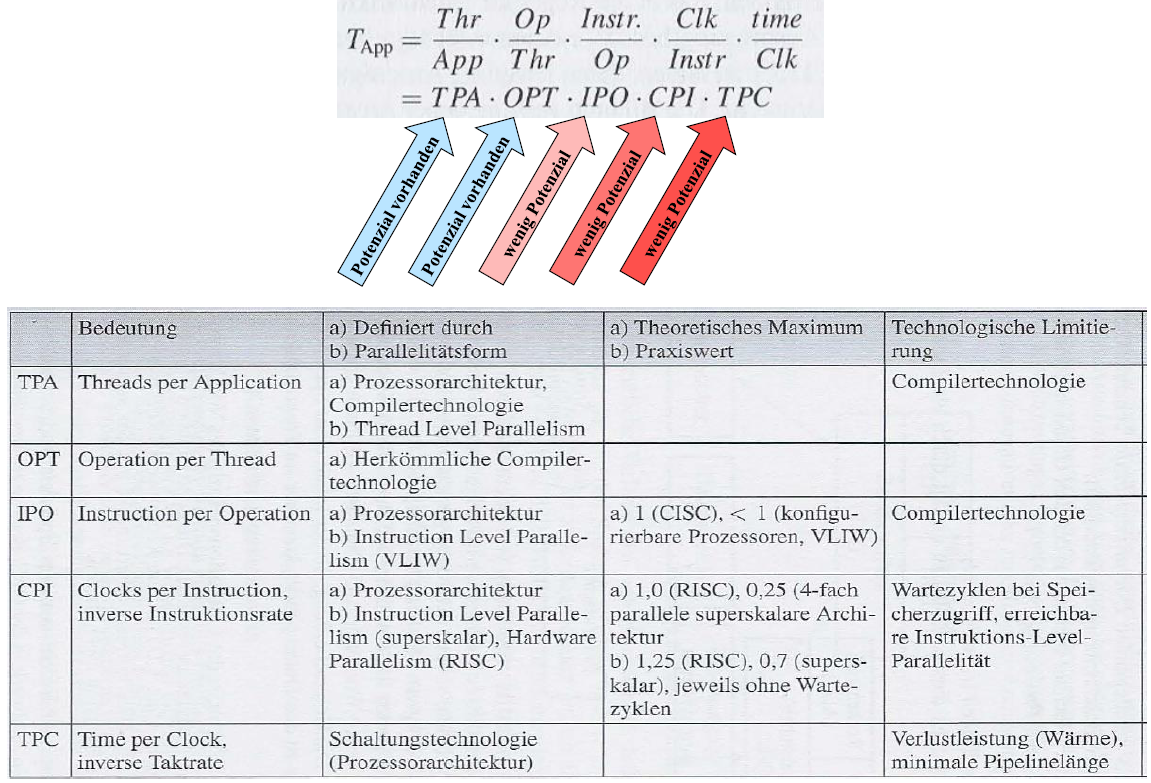
\includegraphics[width=8 cm]{images/Rechnerarchitekturen/Prozessorleistung.PNG}
\end{figure}